\exercise{Morse Code}

\paragraph{Explanation:}
To solve the exercise I simply messages to
morse using the \mttext{morse.mat} file.
Added to the cell array, the space value so that I could iterate through the
message easily without a special case.
To replace the chars with the morse equivalent I defined an inline
function \mttext{get\_morse} which I use in the
\mttext{get\_morse\_message} auxiliary function.
Finally, if there is one output value, I convert this morse
representation into a binary array with the required specifications.

For the beep sound effect I use $ cos(2 \pi F t) $ to get a pure
sound. I use this to model a dot and simply extend it using the
binary pulse array.

\paragraph{MATLAB Code:}

\textbf{Encoder}
\begin{tiny}
    \verbatiminput{code/morse_encoder.m}
\end{tiny}

\textbf{Beep}
\begin{tiny}
    \verbatiminput{code/morse_beep.m}
\end{tiny}

\paragraph{Results:}

Added a test in the \mttext{morse\_run.m} file as well as it acting
as the script to generate the sound for \mttext{"MAE - SPRING 2024"}.

\begin{figure}[H]
    \centering
    \includesvg[width=8cm]{figures/ex1.svg}
    \caption{Sound Waveform}
    \label{fig:figures/ex1.svg}
\end{figure}

Note how fast it oscillates, pretty hard to gather any meaning!
Also compared using $ 4000Hz $ and $ 8000Hz $ as the sampling
frequency, and the sound is indeed sharper at $ 8000Hz $.

\paragraph{Comments:}
I discovered the \mttext{kron} function which I have found very
useful. Also ended using it in the following exercise.

\bigskip
\hrule

\exercise{Koch Fractal Curve}

\paragraph{Explanation:}
I started out implementing the \mttext{koch} function and when I
continued to \mttext{genkoch} I realised a couple of things,
\begin{enumerate}
    \item I could more or less utilise the code I had already done.
    \item I could use \mttext{genkoch} in \mttext{koch} to reduce
        duplicate code.
\end{enumerate}
So that is what I ended doing and therefore will be explaining the
code for \mttext{genkoch} as for the first function I simply create a
triangle, an adequate pattern and call \mttext{genkoch}.

Due to how I started implementing \mttext{koch} I first removed the
first and last dots from the pattern, mainly because these already
exist in the previous iteration.
I then compute the desired separation between plots, which I simply
defined as the $ y $ axis difference in the pattern added to that of
the $ M0 $ and multiplied by $ 1.5 $, just in case.
A smarter and more exact separation could be defined looking at the
potential highest size of the figure, however I deemed it not worth it.

I then iterate through $ n $ and each time use the affine
transformations in the statement for the new points.
I simply had to correctly define all the involved vectors.

To generalise \mttext{koch} I had to replace a couple values I
had hard coded (like the separation between previous points) to get
\mttext{genkoch}.

\paragraph{MATLAB Code:}

As mentioned, my final implementation of \mttext{koch.m} depends on
\mttext{genkoch.m} and therefore will only show the latter.

\begin{tiny}
    \verbatiminput{code/genkoch.m}
\end{tiny}

\paragraph{Results:}

\begin{figure}[H]
    \centering
    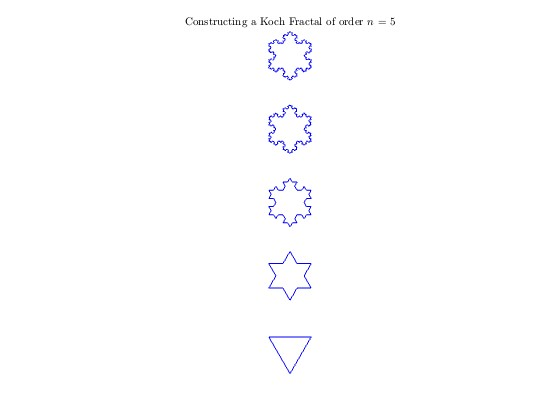
\includegraphics[width=10cm]{figures/koch.jpg}
    \caption{Koch Fractal}
    \label{fig:figures/koch.jpg}
\end{figure}

\begin{figure}[H]
    \centering
    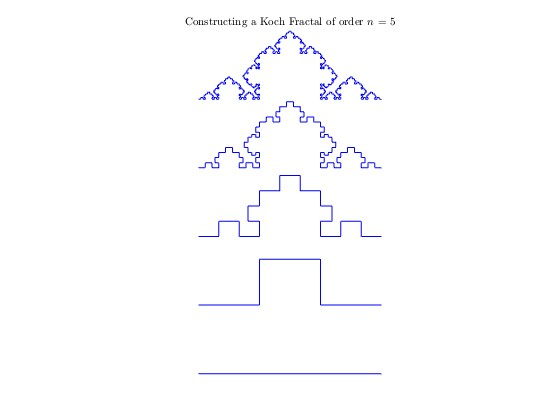
\includegraphics[width=10cm]{figures/genkoch.jpg}
    \caption{Example GenKoch call}
    \label{fig:figures/genkoch.jpg}
\end{figure}

\paragraph{Comments:}

I was initially understanding \textit{affine} transformation as
simply a translation + rotation and was manually resizing the \textit{koch
pattern}, I attached an image below because I though the effect was funny!

\begin{figure}[H]
    \centering
    \includesvg[width=15cm]{figures/small_peaks.svg}
    \caption{Small peaks}
    \label{fig:figures/small_peaks.svg}
\end{figure}

\bigskip
\hrule

